\documentclass[11pt]{article}
\usepackage[margin=1in]{geometry}
\usepackage{graphicx}
\usepackage{amsmath}
\usepackage{microtype}
\usepackage[hidelinks]{hyperref}

\newcommand{\Faq}{\textit{F.~aquilonia}}
\newcommand{\Fpo}{\textit{F.~polyctena}}
\newcommand{\Fst}{\ensuremath{F_{\mathrm{ST}}}}
\newcommand{\dxy}{\ensuremath{d_{xy}}}

\title{\vspace{-3em}Genomic architecture of ancestry sorting:\\
diagnostic index, not recombination, governs its direction}
\author{}
\date{}

\begin{document}
\maketitle
\vspace{-4em}

\noindent\textit{Draft results summary (Module B). Methods are deferred to
Supplementary Materials. All findings are descriptive: any recombination effect
awaits the recombination-matched neutral null, because a non-recombining
autosomal block does not have lower $N_e$ than its surroundings under
neutrality.}

\section*{Results}

\paragraph{Diagnostic index is separable from recombination and reflects reduced
diversity.}
Across the genome the diagnostic index (DI) is essentially orthogonal to the
map-interpolated recombination rate (Spearman $\rho = -0.03$) and to pooled
parental minor-allele frequency ($\rho = -0.02$), making it a genuinely
independent predictor of sorting. Its dominant correlate is \emph{low}
within-species diversity ($\rho = -0.46$ with $\pi$), not elevated absolute
divergence ($\rho = +0.13$ with \dxy), so DI is largely a reduced-diversity
differentiation signal rather than a divergence-island one. A classical
differentiation-island signature---jointly elevated \Fst{} and \dxy{}, reduced
$\pi$, and very large linkage blocks---is confined to the lowest-recombination
decile (Fig.~\ref{fig:mb}a), yet DI is flat across recombination and does not
track it. DI and recombination are therefore separable axes.

\paragraph{Sorting is depleted, not enriched, in low-recombination regions.}
At the independent-unit level, the fraction of units that sort is
\emph{lowest} in the least-recombining decile ($0.06$ versus $\sim\!0.42$
elsewhere; Fig.~\ref{fig:mb}b), because those regions consist of a few very large
linkage blocks whose consensus washes out. The higher SNP-level value in that
decile ($0.17$) relative to the unit level ($0.06$) is spatial pseudo-replication:
adjacent, redundant SNPs in a single low-recombination block. Consistently,
sorting magnitude \emph{increases} with recombination
($\text{prop\_fixed}\sim\text{recombination}$, standardised slope $+0.05$,
$z=117$). Sorting is thus not concentrated where recombination is low---contrary
to a naive linked-selection expectation, and consistent with neutral
book-keeping (fewer independent units per low-recombination block) pending the
null.

\paragraph{Direction is governed by diagnostic index; recombination adds only a
weak independent pull.}
In a logistic model of sorting direction among unidirectional units,
$P(\text{aquilonia}) \sim \text{DI} + \text{recombination} +
\text{parental MAF} + \log(\text{block size})$, diagnostic index dominates
(standardised coefficient $+1.46$, $z=125$): high-DI units fix toward \Faq,
low-DI toward \Fpo, reproducing the Module~A polarity. Recombination contributes
a small but significant independent effect in the opposite-to-expected-noise
direction---low recombination leans \Faq{} after DI, parental MAF and size are
controlled (coefficient $-0.09$, $z=-7.6$)---a modest linked-selection lead. It
is, however, roughly sixteen-fold weaker than DI, and at the raw unit level
direction is nearly flat across recombination (Fig.~\ref{fig:mb}c); the stronger
low-recombination \Faq{} excess seen at the SNP level is largely
pseudo-replication that flattens once independent units are counted.

\paragraph{Outlook.}
Module~B establishes that the predictable polarity of ancestry sorting is
organised by locus diagnosticity, a reduced-diversity axis orthogonal to
recombination, and that sorting is depleted rather than enriched in
low-recombination regions once pseudo-replication is removed. A weak residual
low-recombination pull toward \Faq{} survives control for DI---a lead for the
intrinsic (linked-selection / incompatibility) hypothesis. Adjudicating it
requires the recombination-matched, haplodiploid neutral null; the intrinsic and
extrinsic drivers are then discriminated, respectively, by among-population
linkage disequilibrium between unlinked diagnostic units and by overlap with
climate genotype--environment outliers.

\begin{figure}[h]
\centering
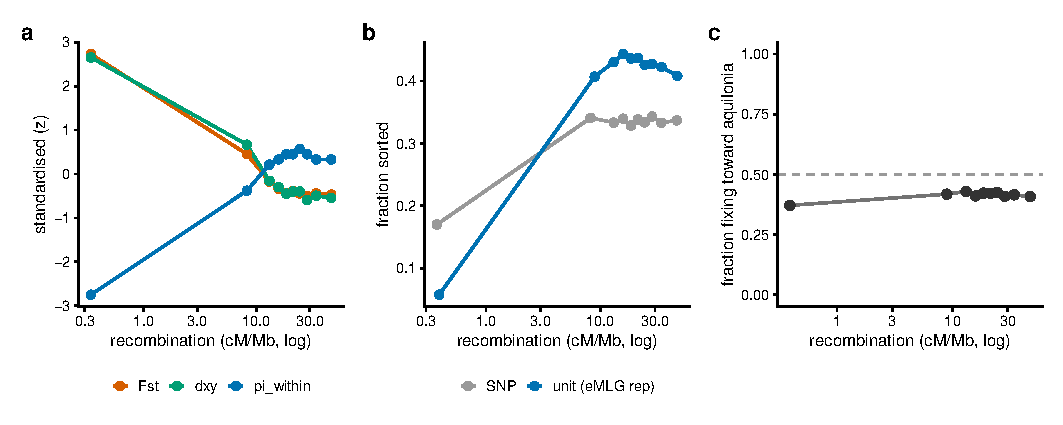
\includegraphics[width=\textwidth]{../Figures/moduleB_fig2.pdf}
\caption{\textbf{Genomic architecture of sorting.}
(\textbf{a}) Standardised relative differentiation (\Fst), absolute divergence
(\dxy) and within-species diversity ($\pi$) across recombination deciles: the
differentiation-island signature is confined to the lowest-recombination decile.
(\textbf{b}) Fraction of loci sorted versus recombination at the SNP level and at
the independent-unit level; the unit-level collapse in low recombination is the
removal of spatial pseudo-replication. (\textbf{c}) Direction of unidirectional
sorting (fraction fixing toward \Faq) versus recombination at the unit level: the
diagnostic-index polarity is not mirrored by a recombination gradient.}
\label{fig:mb}
\end{figure}

\end{document}
